\documentclass[letterpaper]{acm_proc_article-sp}
\usepackage[pass]{geometry}
\usepackage{graphicx}
\usepackage{mathtools}
\usepackage{color}
\usepackage[utf8x]{inputenc}
\usepackage{parskip}

\setlength{\parindent}{0pt}
\setlength{\parskip}{\baselineskip}

\begin{document}

\title{Access Control Policy Verification and Repairing in Alloy}

\numberofauthors{1}

\author{
\alignauthor Alexandr Murashkin, Ming Matthew Ma \\
       \affaddr{The David R. Cheriton School of Computer Science}\\
       \affaddr{University of Waterloo}\\
       \affaddr{Waterloo, ON, Canada}\\
       \email{\{amurashk, m22ma\}@uwaterloo.ca}
}
\date{14 December 2012}
\maketitle

\begin{abstract}

Databases can store important information that may be accessible in non-intended way. Therefore, data access control becomes significant \cite{Fisler:2005:VCA:1062455.1062502}. To express access control policies, several languages such as XACML \cite{oasis:xacml} are used to specify whether subjects are allowed to access sets of resources or services to perform specific actions on them. 

In this paper, we address the problem of verification and repair of access control policy specification\footnote[1]{We use the term "specification" rather than ``model" to avoid ambiguity}. We develop a tool based on first-order logic modeling to detect and display possible conflicts within sets of access control policies expressed in XACML. We first translate the specification into a relational first order logic language called Alloy \cite{jackson:alloy}, and then analyze interactions and conflicts among access control policies using Alloy Analyzer. We then propose potential repairs to the user through the user interface, and automatically apply the fixes selected by the user. We have shown that our tool can automatically determine inconsistencies in user supplied specification, evaluate possible fixes and successfully apply the selected repairs to the specification. 

\end{abstract}

\category{D.2.4}{Software Engineering}{Software/Program Verification}[formal methods]
\category{H.5.2}{Information Interfaces and Presentation}{User Interfaces}[Graphical user interfaces (GUI)]

\terms{Computer Aided Verification, Access Control Policy, Verification, Repair}

\keywords{access control policy, Alloy, XACML, GUI} % NOT required for Proceedings

\section{Introduction and Motivation}

Although XACML has already achieved a considerable degree of industrial acceptance \cite{acp:alloy}, managing access control policies is still error-prone and complicated \cite{acp:automated}. ``Nowadays data is increasingly available on-line through the web and other distributed protocols. This heightens the need to carefully control data access" \cite{Fisler:2005:VCA:1062455.1062502}. For example, students should be able to view their marks, but they are not allowed to modify their marks. This is the responsibility of professors, and they have to be able to modify student marks as well as view them. All such rules are defined within access control policies.

However, ``access control means not only preventing the leakage of data but also permitting access to necessary information" \cite{Fisler:2005:VCA:1062455.1062502}. Therefore, faults in access control policies that allow students to modify their grades or restrict the access of professors to doing that are both dangerous.

The larger the system, the more complicated access control is required. Moreover, in big systems, access control policies may be defined in multiple locations, they are being refined by different people several times. Therefore, it is hard to keep track of all consequences \cite{Fisler:2005:VCA:1062455.1062502}. This, in turn, makes the error localization hard.

Even if an error is localized, there can be many ways to repair access control policy. Manual repairing without tool support is complex and error-prone. We will justify this problem in the following section and show in this paper that such inconsistencies can be detected and fixed automatically using our tool.

\subsection{Problem Statement}

The process of verifying and repairing of access control policies is time-consuming, and development of verification tools like Margrave \cite{Fisler:2005:VCA:1062455.1062502} is good evidence of that. Once inconsistencies are found, the user has to think on how to repair policies, but there is no guarantee that the fixes can indeed repair the specification without introducing new inconsistencies. Thus, the entire process of defining, finding inconsistencies and repairing can be overwhelming for the user.

In this paper, we propose a tool we developed that can automatically determine inconsistencies (or faults), recommend the repair to the users and automatically apply fixes to the access control specification for a subset of XACML.

\subsection{Paper structure}

In the \textit{Background} section we provide relevant information on verification and repair, XACML and Alloy.

All related work we considered is listed in \textit{Related work} section. 

\textit{Theoretical approaches} section will introduce verification and repair approaches we used for our tool. 

In the \textit{Implementation} section we will present the components of our tool and its implementation at different stages. 
\textit{Evaluation} section contains our toy experiment results. In \textit{Future work} section, we discuss our tool limitations and bring up possible future improvements. Conclusion section summarizes completed work and achieved results.

\section{Background}

In this section, we introduce verification and repair, XACML standard for defining access control policies and the Alloy language that we used for verification in our work.

\subsection{XACML access control policies}

XACML is OASIS standard and stands for eXtensible Access Control Markup Language \cite{oasis:xacml}. It defines structure, interaction and conventions related to policy sets, policies, rules and request within an access control system. In our work we use a simplified subset of XACML used in \cite{acp:alloy}. In our case, policy set is a set of policies composed using policy combining algorithm, which can be \textit{PermitOverrides}, \textit{DenyOverrides} or \textit{OnlyOneApplicable}\footnote[2]{we do not consider \textit{FirstApplicable} defined in the XACML standard \cite{oasis:xacml} since it will introduce ordered relations and make our specification more complicated. We also omit dashes and use capitalization for consistency with our specificationl}. Each policy contains the set of rules and rule combining algorithm which can be \textit{PermitOverrides} and \textit{DenyOverrides}. Each request contains one subject, one action and one resource (Fig. \ref{fig:model}), and the system calculates the response of applicable rules, policies, and can make desicions based on that. 

\begin{figure}[h]
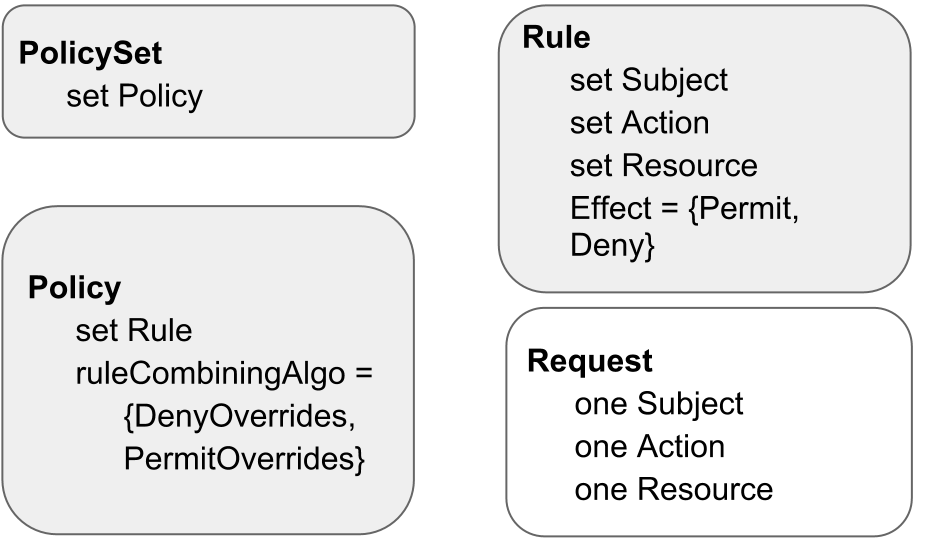
\includegraphics[width=0.5\textwidth]{model.png}
\caption{Shortened representation of some XACML entities: policy set, policy, rule, and request. Alloy-friendly notation}    
  \label{fig:model}
\end{figure}

A decision can be \textit{Permit}, \textit{Deny} or \textit{NotApplicable}; the latter says that the request is not handled by certain rule, policy or policy set. 

Usually XACML access control policies are stored in XML files. For ease of discussion we print XACML policies in a tabular format in this paper, see Fig.\ref{fig:policyset}.

\begin{figure}[h]
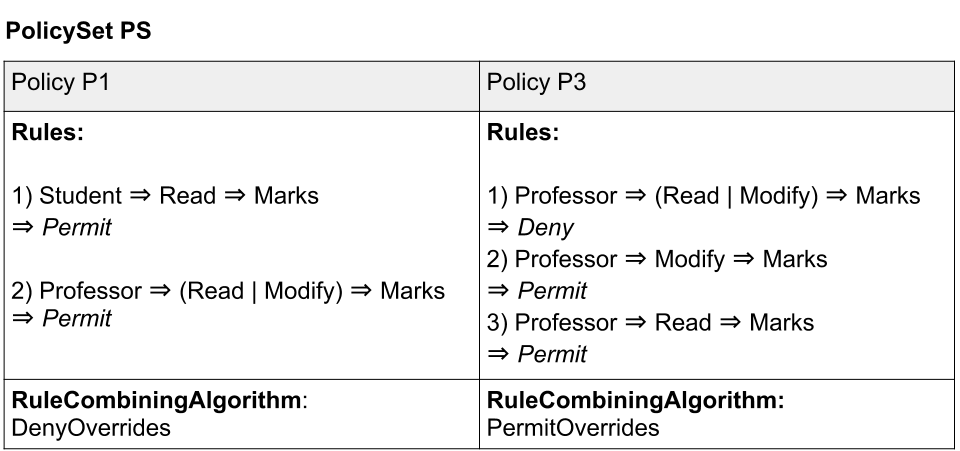
\includegraphics[width=0.5\textwidth]{policyset.png}
\caption{Valid policy set PS contains two policies: P1 and P3, each has a set of rules and rule combining algorithm. In policy P3, the second and third rules are dominant to the first one because of the rule combining algorithm}    
  \label{fig:policyset}
\end{figure}

So, in our example of a consistent policy set (Fig.\ref{fig:policyset}), a policy set $PS$ contains two policies: $P1$ and $P3$, the first rule of $P1$ is $Student \Rightarrow Read \Rightarrow Marks \Rightarrow Permit $ is applied when the subject has the role $Student$, the resource is the $Marks$ file and the action is $Read$, and this access is granted ($Permit$). In policy $P3$, the first rule denies both reading and modifying marks for professor. The policy has $PermitOverrides$ rule combining algorithm which says that this rule is dominated by others in case that more than one rule is applicable for some relevant request. The policy response is equal to the response of the rule which is the only applicable, or by the response of dominant rule if multiple rules are applicable. The same is true for policy set response, but it has $OnlyOneApplicable$ policy combining algorithm as well, which says that the policy set response in indeterministic if more than one policy is applicable in the context of a given request.

\subsection{Verification and repairing}

Given a specification $M$, some property $\varphi$ and satisfaction relation $\models$, verification is the process of determining whether $M\models\varphi$. If $M\not\models\varphi$, the repairing is the process of finding some $M'$, such that $M'\models\varphi$ and $M'$ is derived from $M'$. This derivation should be minimal, but we need to define this criterion and it depends on the domain we consider.

In this paper, we will try to verify and repair specifications that represent access control policies.

\subsection{Alloy}
Alloy \cite{jackson:alloy} is a modeling language based on relational first-order logic. We model concepts in Alloy using so called signatures and relations. An abstract signature operates as a set, type or class definition. For example, we can define a policy as follows (as in \cite{acp:alloy}):
 
 \begin{verbatim}
abstract sig Policy {
  policyTarget : one Target,
  rules : set Rule,
  combiningAlgo : one RuleCombiningAlgo
} 
\end{verbatim}

The keyword \textit{extends} can operate like instantiation of a class, and we can define atom (an atomic signature) that ``extends" another signature (actually, the former becomes an atomic element of the set of the latter \cite{jackson:alloy}). So, Policy1 becomes an instance of Policy:

\begin{verbatim}
one sig Policy1 extends Policy {}{
  policyTarget = T0
  rules = Policy1_Rule_Student_Read_Marks_Permit 
    + Policy1_Rule_Professor_ReadModify_Marks_Permit
  combiningAlgo = DenyOverrides
}
\end{verbatim}

A relation is a set of tuples that relates atoms \cite{jackson:alloy}. In our example, \textit{rules} is relation that relates each policy to a set of rules. Constraints are typically represented in Alloy as global or local facts. A fact is a logical statement that is assumed to always hold. In our example above, ``assignments" of $policyTarget$, $rules$ and $combiningAlgo$ are indeed local facts.

We can also specify functions that take in atoms and return other atoms. In our case, we define such functions to calculate policy response with overridden rules. Alloy also supports predicates that return $true$ or $false$ depending on their input parameters.

The Alloy Analyzer is a tool that takes the specification in the Alloy language and finds variables that satisfy them. It can be used both for specification exploration and verification. The way it works in our case we describe in section \ref{sec:verification}.

\section{Related work}

Regarding access control policy verification, there are several various related approaches.
\cite{Hughes:2008:AVA:1459278.1459282} proposed encoding XACML access control policies  ordering relations and then translation of them into SAT solver for verification. This paper defined some Alloy notation as well.  The papers \cite{acp:automated} and \cite{acp:alloy} defined XACML access control policies notation in Alloy and deal with verification problem. The latter approach - \cite{acp:alloy} - is used in our paper, it introduces the usage of predicates for access control policy verification and validation. We found the way the specifications are defined in this paper straight-forward and easy for repair task, so we used this approach and extended it. Other than that, \cite{4258517} describes inconsistency checking in role-based access control policies (RBAC). \cite{Fisler:2005:VCA:1062455.1062502} proposes Margrave - a tool for access control policies (XACML and other formats) verification and change-impact analysis. \cite {acp:descriptionlogics} used description logics to formalize and verify access control policies. The authors also specified semi-automated access control policy repair as their future work.

None of the paper above solves the problem of access control policy repairing. It does not seem to be published prior related work exactly in this topic and this domain. Rather than that, \cite{Zhang:2004:SVA:1029133.1029141} offers access control policies verification in the language called RW and then synthesize verified specifications in XACML. \cite{Bravo:2007:RIX:1783534.1783545} considers another type of access control policies - XML write access control policies - offers repairs in case of that some actions can be simulated by multiple another actions. Considering different domains, \cite{Reder:2012:CRT:2351676.2351707} proposes repair trees for inconsistency solving in design models. We use similar trees in our repair approaches. There are works on model repairing in temporal logic, but we do not consider the notion of time in our work. Semi-automated repairing of XACML access control policies is the most important contribution of this paper. 

\section{Theoretical approaches}

In this section, we present the verification and repair approaches we use in our work.

\subsection{Verification approach}
\label{sec:verification}

The verification procedure is based on the one in the technical report \cite{acp:alloy}. We use the same idea in our paper and make it more general.
The first step is to define the Alloy input file.

\begin{enumerate}
\item First, an abstract specification  (or meta-model) is defined at the beginning of the file. This abstract specifcation is domain-specific. It consists of signatures ($Policy$, $PolicySet$, $Rule$, $Effect$, $RuleCombiningAlgorithm$, etc.) and relations ($rules$ relation links a policy and rules it contains).

\item Next, a concrete specifcation is defined. It consists of signatures ($Policy1$, $Policy2$, $Rule1$, $Rule2$) and facts ($Policy1$ contains $Rule1$ and $Rule2$) regarding the relations specified in abstract specifcation. Concrete specification can vary within the given domain, so that one abstract specification can be used for many concrete specifcations within the domain.

\item And finally, a property predicate is defined. This predicate is domain-specific as well, and each predicate represents the negation of the property we need to verify. In this paper, we focused on an abstract property: 
\end{enumerate}

\textbf{Property 1}:\textit{Within a policy set that has $OnlyOneApplicable$ policy combining algorithm, there is no two policies that for a given request return different decisions.}

We focused on this property to begin with. Similar property has been specified in \cite{acp:alloy}, but with respect to rules, not policies. However, our approach is not limited to one property: eventually we have to be able to deal with a big set of properties. 

The full body of the predicate that corresponds to the property is given in the Appendix \ref{appendix:A}, and its signature looks as follows:	

\begin{verbatim}
pred InconsistentPolicySet [ps : PolicySet, 
    req : Request,  p1: Policy, p2: Policy, 
    r1: Rule, r2: Rule]
\end{verbatim}

The predicate is supposed to find a policy set $ps$ that has $OnlyOneApplicable$ policy combining algorithm and contains policies $p1$ and $p2$, such that policy $p1$ contains rule $r1$, policy $p2$ contains rule $r2$. At the same time, $r1$ defines the response of policy $p1$: the rule $ r1$ is either the only applicable rule in context of the given request $req$, or dominates all other rules of the policy $p1$ after apllying the rule combining algorithm. And similarly, $r2$ defines the response of policy $p2$.

And the second step is to send the Alloy file to Alloy Analyzer and execute the property predicate. We will denote the part of Alloy file without predicate as a specification (so, the specification consists of two parts: abstract specification and concrete one). If the specification is consistent, then the predicate is inconsistent with respect to the specification, and Alloy Analyzer cannot generate an instance (counterexample). If the predicate is consistent, it means that the specification is inconsistent with respect to the property (the property is not satisfied with respect to the specification), and a counterexample is returned.

\begin{figure}[h]
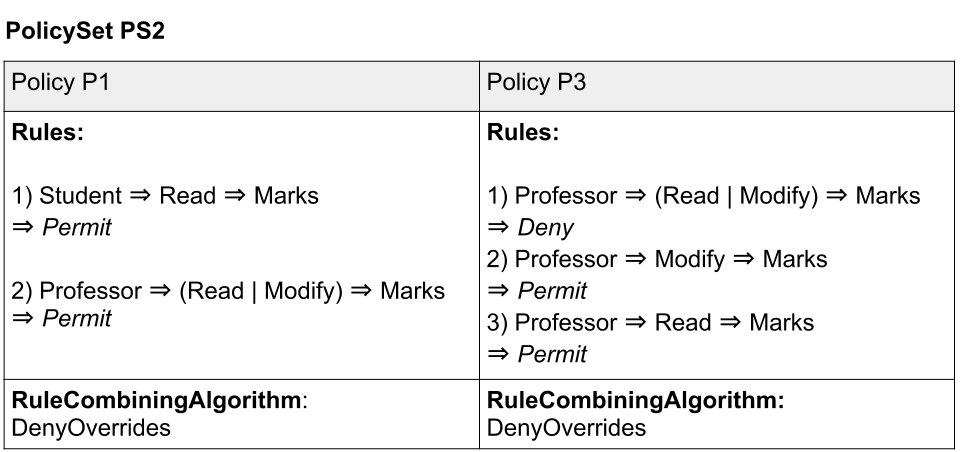
\includegraphics[width=0.5\textwidth]{policyset_faulty.png}
\caption{Faulty policy set PS2. In policy P3, the second and third rules are dominated by the first rule, the rule combining algorithm DenyOverrides says "deny is dominant"}    
  \label{fig:policysetfaulty}
\end{figure}

We consider the example of a policy set PS2 (Fig. \ref{fig:policysetfaulty}) and request $Professor \Rightarrow Read \Rightarrow Marks$. In the context of this request, Policy P1 returns $Permit$, since the only applicable rule is the rule 2 of policy P1. In policy P3, there are two applicable rules: rule 1 which returns $Deny$ and rule 3 that returns $Permit$. Since the rule combining algorithm in policy P3 is $DenyOverrides$, the rule 1 is dominant. Therefore, the response of the policy P3 will be $Deny$. This contradicts with the response of the policy P1, so the policy set PS2 is inconsistent. If we run the verification process in our tool, the variables passed to the predicate will be substituted as follow.  $ps$ is policy set PS2, $p1$ is policy P1, $r1$ is rule 2 of policy P1 ($Professor \Rightarrow (Read|Modify) \Rightarrow Marks \Rightarrow Permit$), $p2$ is policy P3, $r2$ is rule 1 of policy P3 ($Professor \Rightarrow (Read|Modify) \Rightarrow Marks \Rightarrow Deny$), and the request is $Professor \Rightarrow Read \Rightarrow Marks$.

This verification approach gives certain advantages. We can localize the inconsistency, since Alloy Analyzer will show the values of all the arguments of the predicate in the generated instance, including the request $req$, even if there is no definition of request. It is not the case if we make the predicate denote the property itself, not its negation: in this case, if the property is not satisfied, then $UNSAT$ cores can be shown, but it takes computation time to minimize them, and the cores still might not be minimal. So, for error localization the approach we took is better.

\begin{figure*}[ht]
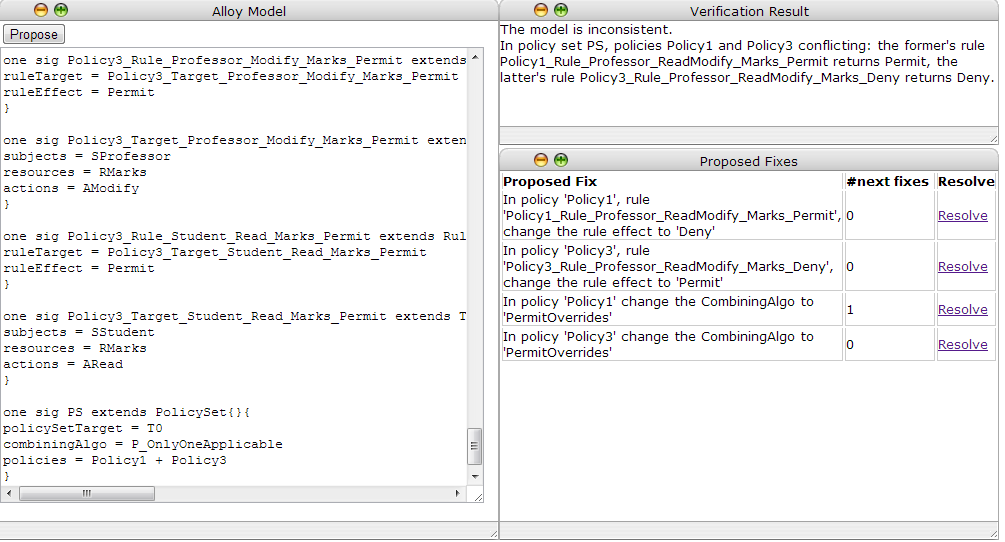
\includegraphics[width=\textwidth]{tool.png}
\caption{Our tool: the User Interface}    
  \label{fig:tool}
\end{figure*}

\subsection{Repair approach}

In this paper we consider repairing of access control policy specifications. We consider a policy set PS2 (Fig.\ref{fig:policysetfaulty}) that is faulty with respect to the same property:

\textbf{Property 1}:\textit{Within a policy set that has $OnlyOneApplicable$ policy combining algorithm, there is no two policies that for a given request return different decisions.}

From PS2, we need to derive a consistent one (there can be many ways of repairing), for example, PS (Fig.\ref{fig:policyset}) is one such an option. Our minimality criterion is defined as the smallest number of changes to the faulty policy specification. But the minimality criterion should be explored in the future work.

Once there is an inconsistent policy set, the verification procedure will return the policy set $ps$, policies $p1$, $p2$ and the corresponding rules $r1$ and $r2$. Our repair procedure is applied to policies or rules, and this will affect the consistency of the policy set $ps$. Since our verification procedure returns two rules of two policies, actually we can try to apply the same set of repairs to each of them by symmetry. Therefore, we can consider the following repair ways in the context of the returned policy set $ps$, and one policy $p1$ and rule $r1$ within it.

\begin{enumerate}
\item Switch the effect of the rule $r1$. If it was $Permit$, it is changed to $Deny$, and conversely.
\item Switch the policy combining algorithm of the policy $p1$. If it was $PermitOverrides$, it becomes $DenyOverrides$, and conversely.
\item Remove the rule $p1$ from the policy $p1$.
\item Remove the policy $p1$ from the policy set $ps$.
\item Switch the policy combining algorithm of the policy set $ps$ from $OnlyOneApplicable$ to either $DenyOverrides$ or $PermitOverrides$.
\item Change subjects, actions or resources of the rule $r1$.
\item Add a new rule to the policy $p1$ that will override current responses of other rules.
\end{enumerate}

The ways 1 and 2 seems to be the best. Just switching the values is definitely less radical. Ways 3 and 4 are dangerous: first, they might affect other requests; next, they can bring us to the empty specification which satisfies everything. Way 5 is quite global to apply it, and again, it will hide the conflicts at all, and this can cause more problems in the future. Other ways like changing rule subjects, actions and resources and adding a new rule should be considered in the future, but in this work they were not implemented, because they are potentially risky and may require more efforts to support. 

So, for this project, we end up with the first two repair ways and we can apply them to both $p1$ and $p2$, so actually we have 4 primitive repair ways:

\begin{enumerate}
\item Switch the effect of the rule $r1$.
\item Switch the policy combining algorithm of the policy $p1$.
\item Switch the effect of the rule $r2$.
\item Switch the policy combining algorithm of the policy $p2$.
\end{enumerate}

However, the application of one repair way might not be enough, in case that the core of inconsistency is not represented by two rules only. First, there might be redundant rules. For example, if the rule $Student \Rightarrow (Read | Modify) \Rightarrow Marks \Rightarrow Permit$ is present, then the rule $Student \Rightarrow Read \Rightarrow Marks \Rightarrow Permit$ is redundant, and changing the rule effect of the latter will cause the application of the former rule and this will not solve the problem in one step. This case is handled during the optimization during the conversion of the source file to Alloy file. Next, there are cases that a policy set is faulty for more than one request (not only for the request $Professor \Rightarrow Read \Rightarrow Marks$, but with the request  $Professor \Rightarrow  Modify \Rightarrow Marks$, for instance), and it definitely needs more than one repair in our approach. This is why we propose the displaying of the approximate numbers of next fixes.

The approximate number of next fixes is calculated as follows. After repairs have been proposed, the system tries to apply each of them gaining partially repaired specifications. Then, the system runs the verification again for each of the partially repaired specifications. If some partially repaired specification is consistent, it means that this specification is fully repaired, and no more repairs needed. So in this case, the number of next fixes is zero. If some partially repaired specification is still inconsistent, then the system tries to apply fixes to the partially repaired specification again, and adds 1 to the number of next fixes. This process can run infinitely and cause state explosion problem, so we limit the depth to certain amount (in our case we specified this depth to be equal to 2).

If the number of next fixes for each fix is greater than zero, then user needs to apply fixes multiple times. The user will go down the repair tree until he will get the fully repaired specification (Fig.\ref{fig:tree}).

\begin{figure}[h]
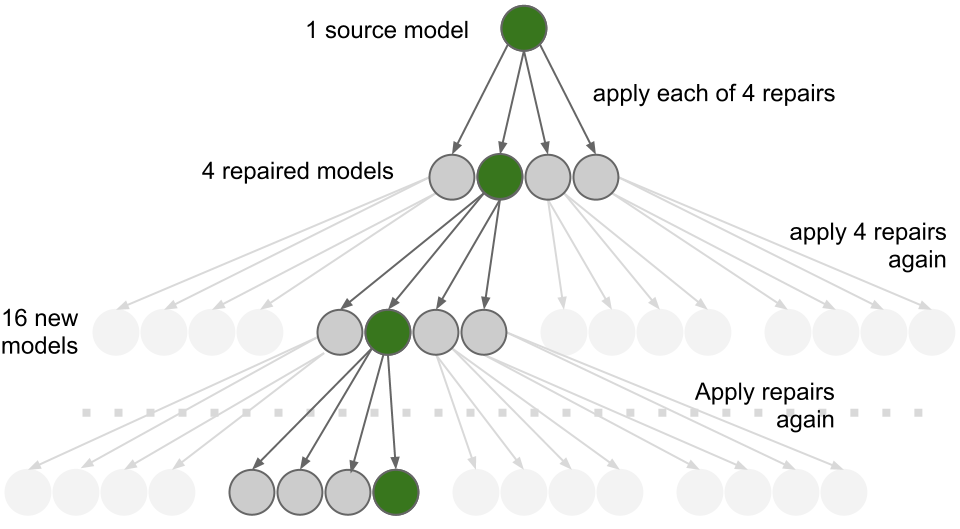
\includegraphics[width=0.5\textwidth]{tree.png}
\caption{Repair trees. Green nodes are decisions of the user. Grey nodes are partially repaired specifications: dark ones are displayed to the user, light ones are precomputed, but not displayed}    
  \label{fig:tree}
\end{figure}

In this approach, more than one path can produce the repaired specification. It does not matter whether this is a minimal one or not: if the user chooses the path with minimal number of next fixes, then eventually he will get the repaired specification with minimal number of changes.

However, there is a problem with this approach - cycles. For example, switching rule combining algorithm may not be helpful. So the system will propose to switch rule combining algorithm and then, at the next step, switch it back. However, our approach helps to solve this problem: if cycles are present, then the way that leads to cycles will be annotated with bigger number of next fixes automatically, so it is less likely that the user will want to choose this way. Still, we can remember last states and detect cycles in another way.

\section{Implementation}
The function of our tool is to automatically determine inconsistencies within access control policy defined by XACML, and recommend the potential repair to the user, and finally apply the user chosen fixes automatically. Throughout this process, user only have to review the recommended fixes, and choose the fix by clicking a button in user interface, and then the specification should be fixed automatically by our tool (Fig. \ref{fig:tool}). 

To increase the usability of our tool, we have implemented external module, a converter that can automatically generate Alloy file based on a table template (or XML, CSV file template) so that the user does not need to know Alloy modeling language. As the content of the such a template, the user is asked to specify the rules, subjects, actions, resources and effects of each rule in predefined format. Our converter will than generate the Alloy file. Once Alloy specification is generated, we input the specification into our inconsistency detection and repair tool. 

\subsection{Architecture and data flow}

Our tool consists of three major parts: the User Interface (UI), PropertyVerifier\&Fixer and Alloy Analyzer. The architecture is shown in the figure below (Fig.\ref{fig:Architecture}).\\

\begin{figure}[h]
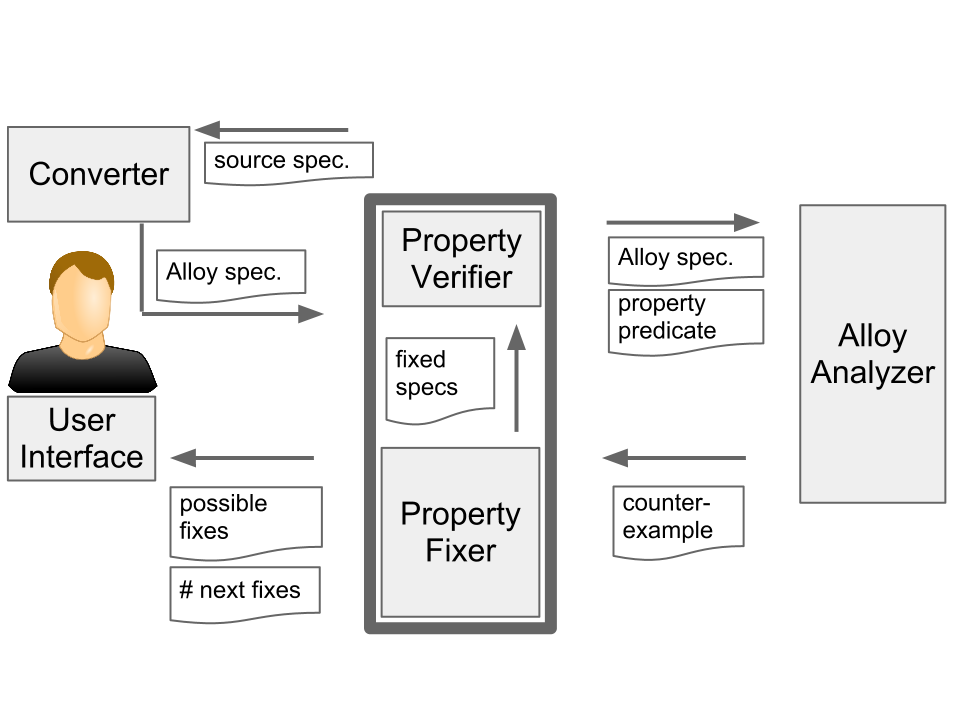
\includegraphics[width=0.5\textwidth]{dataflow.png}
\caption{Tool Architecture and Data Flow}    
  \label{fig:Architecture}
\end{figure}

At the beginning, the UI first takes in the Alloy specification created, and sends it to PropertyVerifier\&Fixer. Next, the PropertyVerifier part starts Alloy Analyzer to processes Alloy specification and its property predicate. It has be noted that we write our predicate in a way that it checks for if two policies return inconsistent results. PropertyFixer then takes in the results from Alloy Analyzer and extracts relevant information, such as inconsistent rules, subject, action, resource and effect, and processes that information to propose the potential fixes. The fix recommendation from PropertyFixer is passed to the UI, and the user is shown with a list of fixes. Once the user chooses one particular fix, our tool will automatically update the original Alloy specification. This updated specification is then passed to PropertyVerifier to check if there are any inconsistencies. This process is repeated until the specification is verified to be consistent.

In order to realize the above mentioned architecture, we have created several Java modules which are summarized below.

\subsubsection{InteractiveRepairer}
This is the core of our tool, it contains:
\begin{itemize}
\item Main engine
\item PropertyVerifier
\item PropertyFixer
\end{itemize}
The Main engine controls the communication between the user interface and our Fixer and Verifier; it processes input from UI and outputs the results to UI for user inspection. PropertyVerifier calls Alloy Analyzer through our API and obtains XML representation of the generated instance that contains information about the policies, rules, request and effects. PropertyVerifier then follows XPath standard to extract and store that information from XML for later processing. Once the XML nodes are extracted with relevant information from Alloy Analyzer, PropertyFixer takes in those information and proposes potential fixes. Once the user selects the preferred fix, this decision is communicated to PropertyFixer again through Main engine, and PropertyFixer will automatically apply the fixes to the original Alloy specification.

Note that PropertyFixer and PropertyVerifier function as a pair, and one pair is required for each property to be verified; in our study, we limit the property verification to the one property but this is extensible by creating another pair of PropertyFixer and Verifier.

\subsubsection{AlloyRunner}
AlloyRunner is an API that facilitate the communication between our tool with Alloy Analyzer. Mainly, it initializes the Alloy Analyzer, sends the specification to Alloy Analyzer, and gets XML instances from it. Alloy Analyzer serves as verification engine for our input specification and will return instances or counterexample which we use in later processing.

\subsubsection{Presentation Layer}
Presentation layer uses dynamic web application technologies such as Javascript and Node.js to allow interactive specification repair. Node.js executes interactive repair with user inputs and calls back to the Main engine in InteractiveRepairer to apply the repair. For instance, the Propose button triggers Main engine to start PropertyVerifier to execute the verification, and the Resolve links will cause the PropertyFixer to apply the repair on the original Alloy specification. The return values are associated with each function call-back of the button, and represents error location and proposed fixes for Propose command and new specification for Resolve command. All proposed fixes are shown and annotated by the approximated number of next fixes.

\section{Evaluation}

Despite XACML is well-adopted standard, we have not evaluated our tool on industry specifications given the time constraints. By now, for our dataset, we have defined 6 toy examples in tabular format. We intentionally made 5 inconsistent examples of policy sets and a consistent one. Policy sets contained from three to four policies with three to six rules each. The tool has successfully identified inconsistent policy sets and proposed the ways of fixing them. The number of next fixes also matched the number we calculated manually. Conducting a proper study with the industry examples is a part of the future work.

\section{Future work}

Although our tool demonstrate potential value in automated access control repair, while significantly reducing user's manual work, we see future improvements in our tool. We noticed the following limitations in our tool:

\begin{enumerate}
\item Verification is bounded
\item Can verify one property in a time until first counterexample is found
\item Subset of XACML is covered
\item Repair procedure depends on the property and requires predefined prospective repair ways
\end{enumerate}

The first two points are pretty clear. Since we use Alloy as it is for bounded verification, we can guarantee that the tool will give correct results within the given scope. Although we significantly dependent on Alloy, we mainly interfaced the communication with Alloy API, so in the future, there will not be problems if Alloy back-end changes.

Although we strive to make our tool scalable, the automated Alloy file generation from a user specified table brings limitations in the structure of the specification we generate. Although this access control specification works well for our present study, it only represents a subset of XACML. In the future, we would like to explore different ways to increase the flexibility of our specification. One potential way is to incorporate sketching techniques and having multiple rule tables so that the user can choose the structure of the specification our tool generates.

Even if the state explosion problem has been handled, it is not addressed in the smartest way due to time constraints. By now, we use repair trees and limit the depth of the potential solution to two. This might still bring problems if the specification is large and the number of fixes is big. We would like to study more on ways to deal better with this common problem in verification and repair.

One important future improvement is on the repair recommendation. Currently, we only propose repairs based on rule effect and combining algorithm. We derived these approach from observation and testing. We will explore other repair ways like changing rule subjects, actions and resources, adding new rules and others to enhance our repair framework. We will also explore possible minimal repair definitions in the domain of access control policies.

And finally, we will conduct more effective evaluation of our tool with industry examples.

\section{Conclusion}

In this report, we presented our tool which can automatically determine inconsistencies in XACML access control policies, recommend possible fixes to the user and automatically apply the repair to the specification. We reduced the manual work, and the tool does not require user knowledge of Alloy as a modeling and verification tool.

We have improved the verification approach and abstract specification presented in \cite{acp:alloy} and proposed repair approach related to this verification approach.

We have implemented the core part of the tool that takes in the Alloy specification and runs Alloy Analyzer in the back-end, and retrieves the information on generated inconsistent instances to propose potential fixes. Among the fixes, it also calculates the approximate number of next fixes required for the selected fix. 

We have designed a user interface of the tool that allows user to input a specification or action and displays verification and repair results. 

From evaluation results, we have shown the feasibility of our approach and that our tool can help the user to repair inconsistent access control policy specifications effectively, requiring only user input for fix selection as a manual part, the rest actions are automated. 

And finally, we have created the input converter so that user can convert policy from other formats. 

\subsection{Implications}

First, we have concluded that semi-automated repair is possible for access control policy defined by XACML structure. 
We have made implications on the fact that user input is still necessary to reduce the complicated computation and steps taken to fixing the specification. By allowing user to select from the list of recommended fixes, we were able to efficiently repair the specification successfully dealing with state explosion.

Next, we have shown that our tool should be easily extensible so that specification repairing is not limited to the property we considered and access control policies domain we addressed. We see our InteractiveFixer module as a ``head'' which we can change according to the specification from another domain or other properties that need to be verified. 


\bibliography{sigproc-sp}{}
\bibliographystyle{abbrv}

\appendix
\section{Verification property predicate} \label{appendix:A}

The predicate below (written in Alloy) is used for automated verification of the following property:

\textbf{Property 1}:\textit{Within a policy set that has $OnlyOneApplicable$ policy combining algorithm, there is no two policies that for a given request return different decisions.}

\begin{verbatim}

pred InconsistentPolicySet [ps : PolicySet, 
    req : Request,  p1: Policy, p2: Policy, 
    r1: Rule, r2: Rule]{

  ps.combiningAlgo = P_OnlyOneApplicable 
  p1 in ps.policies
  p2 in ps.policies
  p1 != p2
  r1 in p1.rules
  r2 in p2.rules
  policyResponse[p1, req] = Permit
  (
    p1.combiningAlgo = DenyOverrides and
    (no r1':Rule | r1' in p1.rules 
      and ruleResponse[r1', req] = Deny)
    and ruleResponse[r1, req] = Permit
  )
  or
  (
    p1.combiningAlgo = PermitOverrides
    and ruleResponse[r1, req] = Permit
  )
  policyResponse[p2, req] = Deny
  (
    p2.combiningAlgo = PermitOverrides and
    (no r2':Rule | r2' in p2.rules 
      and ruleResponse[r2', req] = Permit)
    and ruleResponse[r2, req] = Deny
  )
  or
  (
    p2.combiningAlgo = DenyOverrides
    and ruleResponse[r2, req] = Deny
  )

}

\end{verbatim}



\balancecolumns
\end{document}
